%versi 2 (8-10-2016)
\chapter{Landasan Teori}
\label{chap:teori}
Bab Landasan Teori ini berisi teori yang menjadi dasar eksperimen penelitian ini. \textit{Data Mining} sebagai teori utama yang mendasari penelitian ini. Akan dijelaskan tahap-tahap dari \textit{Data Mining} dan dasar dari \textit{Machine Learning} yang akan digunakan untuk melakukan analisis data terhadap kesuksesan film. Beberapa teknik \textit{preprocessing} juga akan dijelaskan untuk digunakan saat memproses data. 

\section{Penelitian Kaggle}
Sebagai referensi utama dalam penelitian, penulis mempelajari \textit{data mining} dari artikel situs \textit{kaggle} \footnote{Yueming, (2018)\textit{"Analyze IMDB score with data mining algorithms"} https://www.kaggle.com/carolzhangdc/analyze-imdb-score-with-data-mining-algorithms. 8 April 2020.} yang berjudul \textit{"Analyze IMDB score with data mining algorithms"}. Artikel ini membahas penerapan \textit{data mining} pada data film  untuk memprediksi nilai IMDB untuk sebuah film. Terdapat 3 metode yang dibandingkan menggunakan \textit{classification}. Bahasa pemrograman yang digunakan untuk eksperimen adalah R.

Di dalam artikel tersebut, terdapat langkah-langkah \textit{data mining} yang diterapkan. Penelitian dimulai dengan \textit{Data Exploration} untuk memahami data. \textit{Data cleaning} untuk membersihkan data agar dapat digunakan saat \textit{Data mining}. \textit{Data visualization} untuk memvisualisasikan data sehingga mempermudah dalam melihat korelasi dan hubungan tiap data. \textit{Data preprocessing} untuk mengubah data sesuai kebutuhan. \textit{Implement algorithm} untuk memasukkan data yang sudah diproses ke algoritma yang relevan yaitu \textit{classification}. \textit{Classification} merupakan salah satu algoritma \textit{supervised machine learning} yang digunakan untuk memrediksi nilai sebuah kelas.

\textit{Dataset} yang digunakan pada artikel \textit{kaggle} memiliki 5043 data film dengan 28 variabel. Data film berasal dari 100 negara. \textit{Dataset} memiliki 2399 nama sutradara. Nama-nama variabel beserta deskripsinya adalah sebagai berikut :

\begin{itemize}
\item 	\textbf{movie \textunderscore title} : judul film
\item   \textbf{duration}	 : durasi film
\item	\textbf{director \textunderscore name}: nama sutradara 
\item	\textbf{director \textunderscore facebook \textunderscore likes} : jumlah \textit{likes} pada \textit{facebook page} sutradara
\item	\textbf{actor \textunderscore 1 \textunderscore name} : nama pemeran utama 
\item	\textbf{actor \textunderscore 1 \textunderscore facebook \textunderscore likes} : jumlah \textit{likes} pada \textit{facebook page} artis 

\item	\textbf{actor \textunderscore 2 \textunderscore name} : nama pemeran pendukung pertama 
\item	\textbf{actor \textunderscore 2 \textunderscore facebook \textunderscore likes} : jumlah \textit{likes} pada \textit{facebook page} artis 

\item	\textbf{actor \textunderscore 3 \textunderscore name} : nama pemeran pendukung kedua  
\item	\textbf{actor \textunderscore 3 \textunderscore facebook \textunderscore likes} : jumlah \textit{likes} pada \textit{facebook page} artis 


\item \textbf{num\textunderscore user\textunderscore for\textunderscore reviews} : jumlah \textit{user} yang memberikan \textit{review}
\item \textbf{num\textunderscore critic\textunderscore for\textunderscore reviews} : jumlah \textit{user} yang memberikan \textit{critical review}
\item \textbf{num\textunderscore voted\textunderscore user} : jumlah \textit{user} yang mendukung film
\item \textbf{cast\textunderscore total\textunderscore facebook\textunderscore likes} : jumlah \textit{like} dari setiap pemeran film di \textit{facebook}

\item \textbf{movie\textunderscore facebook\textunderscore likes} : jumlah \textit{likes} film di \textit{facebook}
\item \textbf{plot\textunderscore keywords} : kata kunci yang mendeskripsikan film 
\item \textbf{facenumber\textunderscore in\textunderscore poster} : jumlah wajah pemain di poster film 
\item \textbf{color} : jenis warna film ('Black and white' atau 'Color')
\item \textbf{genres}  : kategori film 
\item \textbf{title\textunderscore year} : tahun rilis film (dari tahun 1916 sampai 2016)

\item \textbf{language} : bahasa film 
\item \textbf{country} : negara asal film 
\item \textbf{content\textunderscore rating} : \textit{nilai} konten dalam film 
\item \textbf{aspect\textunderscore ratio} : perbandingan panjang dan lebar layar resolusi film 
\item \textbf{movie\textunderscore imdb\textunderscore link} : tautan film pada imdb 
\item \textbf{gross} : pendapatan kotor 
\item \textbf{budget} : biaya produksi film 
\item \textbf{imdb\textunderscore score} : nilai film yang diberikan oleh imdb 
\end{itemize}

Pada tahap eksplorasi data, beberapa hal dilakukan untuk melakukan \textit{data cleaning} seperti menghilangkan film yang memiliki \textit{missing value}, menghilangkan film yang duplikat, melakukan normalisasi pada judul film. Tahap  eksplorasi dilakukan untuk memahami data dan mengubah data ke bentuk yang lebih relevan untuk tahap pengujian model

Pada tahap visualisasi data, terdapat beberapa teknik yang dilakukan untuk membantu menganalisis data menggunakan grafik seperti memunculkan histogram jumlah film setiap tahun dari 1916 sampai 2016. Pengurutan data dilakukan untuk memunculkan informasi-informasi yang dibutuhkan seperti 20 besar film 
berdasarkan keuntungan dan 20 besar nama sutradara yang menghasilkan film dengan nilai IMDB tertinggi

Eksperimen yang dilakukan pada artikel akan memproses \textit{dataset} yang sudah dibersihkan untuk dimasukkan ke beberapa algoritma \textit{classification} yaitu \textit{Decision Tree}, \textit{K-nearest neighbors} dan \textit{Random Forest}. Berdasarkan hasil pengujian ternyata \textit{Random Forest} memiliki akurasi yang paling tinggi dibanding algoritma lain yaitu 0,76 atau 76 persen. Sehingga, \textit{model} yang dibuat dapat dipercaya untuk memprediksi seberapa bagus film berdasarkan skor IMDB.		

\section{Measuring the Central Tendency  \cite{han2012mining}}\textit{Central Tendency}
 adalah cara untuk mengukur persebaran tiap nilai pada kumpulan data. Kumpulan data yang besar sulit untuk dibaca sehingga membutuhkan suatu cara untuk memahaminya.  \textit{Central Tendency} dapat menghitung sebuah nilai yang dapat merepresentasikan kumpulan data. Terdapat beberapa cara untuk mengukur persebaran data yaitu menggunakan \textit{mean} / rata-rata, \textit{median} (Q2) dan \textit{modus}.  

\subsection{Mean}
\textit{Mean} / rata-rata adalah bilangan yang mewakili sekumpulan data. Rata-rata dapat dihitung dengan menjumlahkan setiap data dibagi dengan jumlah elemen pada data tersebut. Sebuah kumpulan data X dengan elemen x1,x2....xn memiliki N elemen. Berikut adalah rumus \textit{mean} yaitu : 

\begin{equation}
\bar{x} = \frac{\sum_{i}^{N}x_i}{N} = \frac{x1+x2+....+x_N}{N} \
\label{ref:mean}
\end{equation}

X pada Persamaan \ref{ref:mean} merupakan kumpulan data. x1 sampai xn merepresentasikan tiap nilai dari kumpulan data. Penjumlahan dari setiap elemen dapat dibagi dengan jumlah elemen untuk mendapatkan rata-rata dari data tersebut. Untuk mempermudah penjelasan, diberikan contoh yaitu sebuah kumpulan data nilai ujian suatu kelas yaitu 90,85,75 dan 80. Jumlah elemen pada data nilai yaitu 4. Menggunakan \textit{mean} pada \ref{ref:mean}, didapatkan : 

\begin{displaymath}
\bar{x} = \frac{90+85+75+80}{4} \\
= \frac{330}{4} = 82.5
\end{displaymath}


\subsection{Median}
\textit{Median} adalah nilai tengah yang dapatkan dari sebuah data yang terurut. Jika banyaknya data genap, maka rumus mediannnya adalah : 

\begin{equation}
Me(Q2) = \frac{(X_{n/2} + X_{(n/2)+1})}{2}
\label{ref:mediangenap}
\end{equation}
	
$X_n dan X_{n+1}$ pada Persamaan \ref{ref:medianganjil} merupakan data urutan ke $n/2$ yang sudah terurut menaik. Jika banyaknya data ganjil, maka rumus median adalah : 

\begin{equation}
Me(Q2) = \frac{X_{(n+1)/2}}{2}
\label{ref:medianganjil}
\end{equation}

 $X_{(n+1)/2}$ pada Persamaan \ref{ref:medianganjil} merupakan data urutan ke $n/2$ yang sudah terurut menaik. Untuk mempermudah penjelasan, diberikan sebuah contoh yaitu kumpulan data nilai ujian yang sudah terurut menaik yaitu 75,80,85 dan 90. Maka didapatkan perhitungan \textit{median} yaitu :
 
\begin{displaymath}
Me(Q2) = \frac{X_{n/2} + X_{n/2}+1}{2} = \frac{X_{2} + X_{3}}{2} = \frac{80+85}{2} = 82.5
\end{displaymath}

\subsection{Modus}
\textit{Modus} adalah elemen pada kumpulan data yang paling sering muncul. Terdapat beberapa jenis \textit{modus} yaitu \textit{unimodal} , \textit{bimodal} dan \textit{trimodal}.  \textit{Modus unimodal} yaitu elemen dengan frekuensi terbanyak berjumlah 1. Berikut adalah contoh kumpulan data nilai ujian sekolah yang terurut adalah 75,80,85,85 dan 90. \textit{Modus} pada kumpulan data ini adalah 85 karena frekuensi kemunculan elemen 85 adalah 2 kali.  
 
% BAGIAN DATA MINING 
 
\section{Data Mining  \cite{han2012mining}}
\textit{Data Mining} / \textit{Knowledge Discovery Process} (KDD) adalah proses menemukan suatu pola dari kumpulan data yang besar. Dengan \textit{data mining}, manusia dapat menemukan sebuah 
informasi / pemahaman baru dari data. Sumber data objek yang dapat diproses untuk \textit{data mining} adalah dari \textit{database}, \textit{data warehouse} atau data yang didapatkan dari sebuah proses.

Suatu data objek yang digunakan di \textit{data mining} merupakan sebuah entitas. Kumpulan dari data objek disebut \textit{data set}. Contoh nama lain \textit{data set} adalah \textit{data points} dan \textit{objects}. Contoh data objek adalah data pelanggan di salon, transaksi pembelian di supermarket, data pasien di rumah sakit, data mahasiswa di kampus dan lain-lain.

Atribut adalah sebuah karakteristik dan kondisi dari data objek. Data objek dapat memiliki satu atau lebih atribut.  Atribut dapat disebut juga sebagai dimensi, fitur atau variabel. Contoh atribut adalah
sebuah data objek transaksi pembelian di supermarket memiliki kumpulan atribut yaitu \textit{customer\_ID}, \textit{name} dan \textit{address}. Sebuah atribut memiliki beberapa jenis yaitu nominal, biner, ordinal, atau numerik. 

Atribut numerik adalah jenis nilai kuantitatif. Atribut numerik dapat diukur kuantitasnya. Nilai dari atribut numerik dapat berupa bilangan bulat (\textit{integer}) atau bilangan \textit{real}. Atribut numerik dapat dibagi lagi menjadi interval dan rasio.   

Atribut nominal adalah tipe atribut yang tiap nilainya merupakan sebuah kategori/kondisi/kode. Atribut nominal memiliki isi berupa sebuah nama, simbol dari objek yang direpresentasikan. Nilai nominal tidak dapat dipengaruhi oleh perhitungan karena setiap angka/kode menunjukkan kondisi. Contoh atribut nominal adalah sebuah objek data pelanggan supermarket memiliki atribut jenis kelamin yang bernilai 'Pria' atau 'Wanita'.
 
Atribut biner adalah tipe atribut yang serupa dengan nominal tetapi hanya memiliki 2 jenis nilai. Biasanya, nilai biner dikodekan menjadi 0 dan 1. Contoh dari nilai biner adalah atribut pembayaran pada data objek transaksi memiliki nilai \textit{true} atau \textit{false} yang menyatakan pernyataan pembayaran sudah diselesaikan.

Atribut ordinal adalah tipe atribut yang memiliki hubungan keterurutan dari setiap nilainya. Atribut ordinal dapat dihasilkan dari mengubah nilai numerik yang disebut \textit{discretization}. Contoh dari atribut ordinal adalah nilai survei kepuasan penduduk yang awalnya memiliki rentang nilai 0 sampai 10 lalu dikonversikan menjadi ordinal berupa buruk, puas dan sangat puas. 

Berikut adalah ilustrasi gambar proses \textit{Data Mining} yaitu : 


\begin{figure}[h!]
	\centering  
	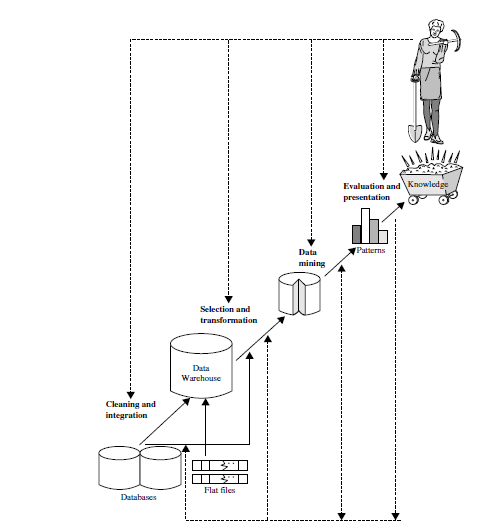
\includegraphics[scale=0.7]{bab2/dataminingprocess}   
	\caption{Proses Data Mining}
	\label{fig:dataminingprocess} 
\end{figure} 

berdasarkan Gambar \ref{fig:dataminingprocess} di atas, berikut adalah penjelasan dari masing-masing proses yaitu :
 
\begin{itemize}
\item \textbf{\textit{Data cleaning}} : menghilangkan noise dan data yang tidak konsisten
\item \textbf{\textit{Data integration}} : menggabungkan data dari beberapa sumber jika ada
\item \textbf{\textit{Data transformation}} :mengubah bentuk data menjadi lebih mudah dan relevan untuk kebutuhan analisis
\item \textbf{\textit{Data selection}} : memilih data yang relevan untuk melakukan analisis
\item \textbf{\textit{Data mining}} :proses menggunakan metode \textit{machine learning} untuk menemukan pola dari sebuah data 
\item \textbf{\textit{Pattern evaluation}} : untuk memeriksa dari pola yang dihasilkan apakah dapat menghasilkan kebenaran mengenai pola yang ditemukan
\end{itemize}


\subsection{Data Cleaning}
\label{chap:datacleaning}
\textit{Data Cleaning} merupakan salah satu tahap \textit{data preprocessing}. \textit{Data cleaning} adalah kegiatan untuk membersihkan data. Data kotor adalah data dengan yang memiliki \textit{missing value}, mengubah atau menghilangkan \textit{noisy data}. \textit{Noisy data} adalah data yang seharusnya tidak berada dikumpulan \textit{dataset}. \textit{Noisy data} dapat muncul dikarenakan beberapa hal seperti kesalahan proses saat perangkat keras membaca data, salah input,\textit{human error} atau kesalahan saat diproses menggunakan perangkat lunak. \textit{Noisy data} harus dihilangkan dikarenakan dapat memengaruhi hasil proses \textit{data mining}.

 Proses \textit{Data Cleaning} membantu analisis data yang lebih valid. Terdapat beberapa cara yang dapat dilakukan jika pada data terdapat nilai yang hilang / \textit{missing value} seperti :

\begin{itemize}
\item \textbf{Mengabaikan bagian data tersebut:} metode ini dapat dilakukan dengan cara mengabaikan \textit{missing value}. \textit{Missing value} dapat diabaikan jika data yang \textit{missing value} tidak terlalu banyak. Sedikit data yang diabaikan tidak akan mempengaruhi hasil \textit{data mining}
\item \textbf{Mengisi nilai yang hilang secara manual:} metode ini tidak dapat direkomendasikan karena prosesnya yang memakan banyak waktu.
\item \textbf{Menggunakan nilai konstan untuk mengisi nilai yang hilang:} \textit{missing value} dapat diubah dengan membuat nilai konstan. Contoh yang dapat dipahami adalah mengubah \textit{value} yang kosong menjadi \textit{'unknown'} pada suatu atribut. Data yang sudah ditandai \textit{'unknown'} akan membantu komputer mengidentifikasinya. 
\item \textbf{Menggunakan nilai tengah:} nilai yang hilang dapat diubah dengan nilai tengah yang tidak akan mempengaruhi distribusi data. Cara yang dapat digunakan adalah mengubah data tersebut menjadi \textit{mean} /rata-rata  dari \textit{data set}.
\end{itemize}


\subsection{Data Integration} 
\label{chap:dataintegration}
\textit{Data integration} adalah proses menggabungkan data dari beberapa sumber data. \textit{Data integration} dapat menghasilkan data baru yang akan membantu proses \textit{data mining}. Kebutuhan baru akan tambahan deskripsi data membuat proses \textit{data integration} perlu dilakukan. Cara yang dapat dilakukan pada tahap \textit{Data integration} adalah menggabungkan beberapa tabel dari basisdata, \textit{web crawling} yaitu mengekstrak data dari \textit{web pages}. 



\subsection{Data Reduction} 
\label{chap:datareduction}
\textit{Data reduction} adalah salah satu \textit{data preprocessing} yang dilakukan untuk mengurangi \textit{data set} menjadi jumlah yang lebih sedikit. \textit{Data reduction} diterapkan untuk mempercepat proses \textit{data mining} dan meningkatkan akurasi dalam proses \textit{data mining}. Metode \textit{Data reduction} dibagi menjadi dua yaitu \textit{dimensionality reduction} dan \textit{numerosity reduction}. 

\textbf{\textit{Dimensionality Reduction}} adalah proses memilih atribut tertentu dan menghilangkan atribut data yang tidak dibutuhkan. Teknik yang dapat dilakukan adalah menggunakan \textit{feature selection}. \textit{Feature selection} adalah teknik untuk memilih atribut yang relevan untuk \textit{predictive analysis} menggunakan \textit{machine learning}.

\textbf{\textit{Numerosity Reduction}} adalah proses memilih baris data tertentu dan menghilangkan sisa baris yang tidak digunakan. Cara yang dapat dilakukan adalah \textit{sampling} yaitu mengambil \textit{subset} dari data secara \textit{random}. \textit{Sampling} akan mengambil sebagian data yang mewakili kumpulan dari \textit{dataset}. 

\subsection{Data Transformation}
\label{chap:datatransformation}
\textit{Data Transformation} adalah proses mengubah data yang lebih sesuai saat digunakan saat proses \textit{data mining}. Terdapat beberapa metode yang dapat digunakan untuk \textit{data transformation} yaitu : 

\begin{itemize}
\item \textbf{Smoothing} : \textit{smoothing} adalah kegiatan untuk memproses \textit{noisy data}. \textit{Noisy data} dapat diproses dengan berbagai cara seperti mengubah menjadi \textit{mean} data tersebut dan mengabaikannya.
\item \textbf{Attribute Construction} : menambah atribut baru berdasarkan atribut yang sudah ada demi membantu proses \textit{data mining}. 
\item \textbf{Aggregation}: menghitung dan menyimpan data laporan seperti nilai maksimum, minimum dan rata-rata dari \textit{data set}
\item \textbf{Normalization}: atribut data tertentu diskalakan pada rentang nilai tertentu yang lebih distandarkan. Normalisasi akan mengubah skala sebuah kumpulan nilai yang ada menjadi rentang 0 sampai 0.1. Salah satu caranya adalah dengan menggunakan \textit{Minmax Normalization}
\item \textbf{Discretization}: proses mengubah atribut numerik menjadi diskret. Contohnya adalah mengubah  atribut 'umur'. Umur dapat diubah menjadi kelompok nilai yang memiliki jarak  berdasarkan jenis. Contohnya adalah 'balita' direntang 2-5 tahun, anak kecil direntang 5-12 dan 'remaja' rentang 12-17 tahun. 
\end{itemize}


\subsection{Data Selection}
\label{chap:dataselection}
\textit{Data Selection} adalah proses memilih data yang tepat untuk melakukan analisis dengan \textit{machine learning}. Sebuah \textit{data set} memiliki dua atau lebih atribut. Data perlu dipilih dengan mengambil atribut yang relevan dan mengabaikan atribut yang tidak relevan. \textit{Machine Learning} akan melakukan prediksi nilai atribut yang disebut \textit{response} / dependen berdasarkan atribut prediktor/independen Pemilihan atribut yang tepat akan meningkatkan akurasi dalam pembuatan \textit{model}. Terdapat beberapa teknik yang dapat digunakan untuk memilih fitur/prediktor yang tepat.

\subsubsection{Pearson Correlation}
\label{chap:teori_pearsoncorrelation}
\textit{Pearson Correlation} adalah teknik yang dapat digunakan untuk memeriksa korelasi antara 2 atribut numerik yaitu A dan B. Berikut adalah rumus dari penghitungan koefisien korelasi : 

\begin{equation}
^r A,B = \frac{\sum_{i=1}^{n}(ai - \overline{A})(bi - \overline{B})}{n\sigma A \sigma B}
\label{eqref:pearsoncorrelation}
\end{equation}

Persamaan \ref{eqref:pearsoncorrelation} adalah rumus \textit{pearson}. $n$ adalah jumlah baris, $ai$ dan $bi$ adalah nilai A baris i dan nilai B baris i, $ \overline{A} $  dan $\overline{B}$ adalah nilai rata-rata dari A dan B, $\sigma A$ dan $\sigma B$ adalah nilai standar deviasi dari A dan B. Jika hasil perhitungan koefisien korelasi lebih dari 0, maka A dan B memiliki hubungan \textbf{korelasi positif}. Hubungan korelasi positif adalah kondisi ketika naiknya nilai A maka nilai B juga akan naik. 

Jika hasil perhitungan koefisien korelasi adalah 0, maka A dan B adalah atribut \textbf{independen} dan tidak memiliki korelasi. Jika hasil perhitungan koefisien korelasi adalah lebih kecil dari 0, maka A dan B memiliki hubungan \textbf{korelasi negatif}. Korelasi negatif adalah hubungan dimana ketika satu atribut nilainya semakin bertambah, maka atribut lain akan berkurang. \textit{Scatter plot} juga dapat digunakan untuk melihat korelasi antara 2 atribut.  


\subsubsection{Chi Square ($X^2 $)}
\textit{Chi Square} adalah teknik yang dapat digunakan untuk memeriksa korelasi antara 2 atribut kategori. Berikut adalah rumus dari perhitungan \textit{chi square} yaitu : 

\begin{equation}
X_{c}^{2} = \sum \frac{(O_i - E_i)^2}{E_i}
\label{eqref:chisquare}
\end{equation}

Persamaan \ref{eqref:chisquare} adalah rumus untuk menghitung \textit{chi Square}. C adalah tiap kejadian atribut respon dan prediktor. $O_i$ adalah jumlah \textit{observed value} yaitu jumlah kemunculan prediktor i pada respon i. \textit{Expected value} dapat dihitung dengan :

\begin{equation}
E1 = n * p 
\end{equation}
\begin{equation}
p = P(predictor_i) * P(response_i) 
\label{eqref:expectedvaluechisquare}
\end{equation}

Persamaan \ref{eqref:expectedvaluechisquare} adalah perhitungan untuk mendapatkan nilai \textit{Expected}. Penjumlahan dari setiap perhitungan kemungkinan pasangan atribut prediktor dan respon akan menjadi \textit{chi square}. Semakin tinggi nilai \textit{chi square}, maka semakin relevan sebuah pasangan atribut prediktor dan respon digunakan.


\section{Machine Learning  \cite{tan_steinbach_karpatne_kumar_2020}} 
\textit{Machine Learning} adalah metode yang dapat dilakukan komputer untuk belajar berdasarkan data. Dengan \textit{Machine Learning}, komputer dapat mengambil sebuah keputusan atau memprediksi. Komputer akan mencari pola dari kumpulan sampel data yang disebut dengan \textit{training data}. \textit{Machine learning} juga disebut sebagai \textit{predictive analysis} karena dapat membantu komputer untuk mengambil sebuah keputusan. \textit{Machine Learning} dapat dibedakan berdasarkan jenis \textit{input} dan \textit{output} yang dihasilkan. Jenis-jenis kategori \textit{Machine Learning} yaitu :  
		
		\begin{itemize}
			\item \textit{\textbf{Supervised Learning}} : algoritma yang  menerima kumpulan sampel data yang dijadikan \textit{training data} dan menghasilkan \textit{output} berupa jenis kelas dari data tersebut. \textit{Supervised learning} menerima data yang sudah memiliki label agar dapat memrediksi data baru berdasarkan \textit{training data}. Algoritma \textit{supervised learning} antara lain adalah \textit{Regression} dan \textit{Classification}. \textit{Supervised learning}  disebut sebagai \textit{predictive analysis} karena kemampuannya untuk memprediksi nilai 
			
			\item \textit{\textbf{Unsupervised Learning}} : algoritma yang menerima kumpulan sampel data \textit{training} yang belum memiliki label. \textit{Unsupervised learning} dapat digunakan untuk mengelompokkan kumpulan data berdasarkan nilai dan kesamaan. Algoritma \textit{unsupervised learning} adalah \textit{clustering}. \textit{Unsupervised Learning} disebut sebagai \textit{descriptive analysis} karena kemampuannya untuk mengelompokkan data sesuai kemiripan dan mendeskripsikannnya. 
		\end{itemize}	


\subsection{Regression  \cite{draper_smith_1998}} 
 \textit{Regression} adalah  teknik \textit{supervised learning} yang digunakan untuk memprediksi nilai kontinu. Regresi menerima sampel data numerik sebagai input untuk menghasilkan sebuah persamaan yang dapat digunakan untuk memprediksi nilai yang dibutuhkan. Regresi memrediksi nilai variabel bergantung (\textit{response}) berdasarkan nilai variabel  independen. Terdapat beberapa jenis \textit{regression} yaitu \textit{linear regression} dan \textit{polynomial regression}.
		
%		MACHINE LEARNING -> SUPERVISED -> REGRESSION -> LINEAR REGRESSION 
\subsubsection{Linear Regression}   
Linear Regression adalah algoritma regresi yang digunakan untuk menghasilkan persamaan linear. \textit{Linear regression} juga dapat digunakan untuk menguji sejauh mana hubungan sebab akibat antara variabel dependen dengan variabel independen. \textit{Linear Regression} dapat digunakan untuk memrediksi nilai kontinu. Persamaan \textit{linear regression} yaitu : 
		
\begin{equation}
 Y = a + bX
\label{eqref:linearregression}
\end{equation}


	
Nilai Y pada persamaan \eqref{eqref:linearregression} merupakan atribut variabel dependen (\textit{response}). X merupakan atribut variabel independen (\textit{predictor}). a merupakan konstanta dan b merupakan koefisien regresi (kemiringan). Koefisien regresi merupakan besaran \textit{response} yang ditimbulkan oleh \textit{predictor}. Nilai-nilai a dan b dapat dihitung dengan menggunakan rumus yaitu : 
		
		\begin{equation}
		 a = \frac{(\sum_{}^{} y)(\sum_{}^{} x^2) - (\sum_{}^{} x)(\sum{}^{} xy)}{n(\sum{}^{} x^2)-(\sum{}^{} x)^2}   
		 \label{eqref:konstantalinearregresi}
		\end{equation}
		\begin{equation}
		b = \frac{n(\sum{}^{} xy)-(\sum{}^{} x)(\sum{}^{} y)}{n(\sum{}^{} x^2)-(\sum{}^{} x)^2}
		\label{eqref:koefisienregresi}
		\end{equation}

Berdasarkan uraian rumus \eqref{eqref:koefisienregresi} dan rumus \eqref{eqref:konstantalinearregresi}, seberapa kuatnya pengaruh variabel atribut independen terhadap variabel  atribut dependen dapat dihitung menggunakan koefisien determinasi ($\mathbf{R^2}$).



		
%		MACHINE LEARNING -> SUPERVISED -> REGRESSION -> POLYNOMIAL REGRESSION 
\subsubsection{Polynomial Regression}
 \textit{Polynomial Regression} adalah algoritma \textit{regression} yang digunakan untuk menghasilkan persamaan polinomial (suku banyak) berdasarkan data yang diinput. Persamaan  akan berubah sesuai dengan \textit{degree} / orde yang ditentukan. Persamaan yang dihasilkan dapat digunakan untuk menghitung nilai variabel bergantung menggunakan nilai variabel independen dan koefisien yang ditemukan. Persamaan \textit{polynomial regression} adalah : 
		
		
		\begin{equation}
		   y = a0 + a_1x + a_2x^2 + .. +  a_n x^n     
		   \label{eqref:persamaanpolinom}
		\end{equation}
		
		
Nilai Y pada persamaan \ref{eqref:persamaanpolinom} merupakan variabel dependen yang ingin diprediksi. Nilai a0 sampai aN adalah nilai koefisien. Nilai X adalah atribut variabel independen. Sebelum menggunakan persamaan di atas, kita perlu untuk mencari koefisien dari setiap suku perpangkatan. Untuk persamaan polinomial orde 2 didapatkan hubungan yaitu : 
		
		
		\begin{equation}
		\begin{cases}
		  
		   	na_0 + (\sum_{i=1}^{n}xi) a_1 + (\sum_{i=1}^{n}xi ^2)a_2 &= \sum_{i = 1}^{n} yi \\
		   		(\sum_{i=1}^{n}xi) a_0 + (\sum_{i=1}^{n}xi^2)a_1 + (\sum_{i=1}^{n} xi^3)a_2 &= \sum_{i=1}^{n} (x_i y_i) \\
		   		(\sum_{i=1}^{n} xi^2)a_0 + (\sum_{i=1}^{n} xi^3)a_1 + (\sum_{i=1}^{n}xi^4)a_2 &= \sum_{i=1}^{n}(x_i^2 y_i)
		   
		\end{cases}
		\label{eqref:hubunganpolinom}
	   \end{equation}
		
Berdasarkan persamaan \ref{eqref:hubunganpolinom}, dapat diubah dalam bentuk matriks persamaan untuk mendapatkan koefisien yaitu : 
		
		\begin{equation}
			\begin{bmatrix}
			n & \sum_{i=1}^{n}xi & \sum_{i=1}^{n}xi ^2 \\
			\sum_{i=1}^{n}xi & \sum_{i=1}^{n}xi^2 & \sum_{i=1}^{n} xi^3 \\
			\sum_{i=1}^{n} xi^2 & \sum_{i=1}^{n} xi^3 & \sum_{i=1}^{n}xi^4
			\end{bmatrix}
			\begin{bmatrix}
			a0 \\ 
			a1 \\ 
			a2
			\end{bmatrix}
			=
			\begin{bmatrix}
				 \sum_{i = 1}^{n} yi \\
				 \sum_{i=1}^{n} (x_i y_i) \\
				 \sum_{i=1}^{n}(x_i^2 y_i)
			\end{bmatrix}
			\label{eqref:matrixpolinom}
		\end{equation}
		
Persamaan \eqref{eqref:matrixpolinom} dapat menemukan masing-masing koefisien sehingga dapat dimasukan pada persamaan \textit{Polynomial Regression}. Hasil perhitungan koefisien dapat diaplikasikan pada rumus persamaan sehingga bisa menghitung prediksi nilai atribut respon (dependen).



\subsubsection{Evaluasi Regresi}
\label{chap:evaluasiregresi}
Sebuah model yang dibuat untuk melakukan prediksi dengan regresi dapat diukur estimasi keakuratan prediksinya. Metode yang dilakukan untuk mengukurnya yaitu nilai \textit{error} dan akurasi. Metode yang dapat digunakan untuk menguji seberapa baik hasil prediksi atribut respon yang ingin diperoleh adalah dengan membandingkan selisih antara atribut respon pada \textit{test set} (y true) dengan atribut respon yang diprediksi (y pred) menggunakan model ini

\paragraph{\textit{Mean Squared Error}}  \mbox{}\\
 Selisih antara prediksi dan yang asli disebut dengan \textit{error}. \textit{Mean Squared Error} (MSE) adalah rata-rata dari nilai \textit{error} setiap data objek. Rumus dari MSE (\ref{eqref:mse}) adalah : 


\begin{equation}
  \frac{1}{N}\sum_{i=1}^{n} (y true_i - y pred_i)
  \label{eqref:mse}
\end{equation}

\textit{Root Mean Squared Error} (RMSE) adalah akar pangkat dari MSE yang akan memberikan nilai yang lebih dapat dinormalkan. Berikut adalah rumus dari RMSE (\ref{eqref:rmse}) yaitu : 

\begin{equation}
 \sqrt{\frac{1}{N}\sum_{i=1}^{n} (y true_i - y pred_i)}
  \label{eqref:rmse}
\end{equation}

\paragraph{Coefficient of Determination (R2)} \mbox{}\\

 \textbf{Koefisien determinasi} adalah nilai yang menunjukkan kuat/tidaknya hubungan antara dua variabel. Berikut adalah cara menghitung koefisien determinasi : 
		
		
		\begin{equation}
		R^2 = 1 - \frac{\sum{}^{}(y-\hat{y})^2}{\sum{}^{}(y-\bar{y})^2}
		\label{eqref:koefisiendeterminasi}		
		\end{equation}
		
Uraian rumus \eqref{eqref:koefisiendeterminasi} di atas merupakan cara untuk menghitung koefisien determinasi.  Y adalah nilai \textit{response} / nilai asli yang ingin diprediksi. $\hat{y}$ adalah hasil prediksi yang dihasilkan oleh model. $\bar{y}$ adalah \textit{mean} dari kumpulan data.

Terdapat 3 kemungkinan dalam hasil perhitungan koefisien determinasi. Jika nilai \textit{$R^2$} > 0, maka kedua atribut memiliki korelasi positif. Korelasi positif  terjadi saat suatu nilai atribut meningkat (X), maka atribut lainnya (Y) juga meningkat. Jika nilai \textit{$R^2$} < 0, maka kedua atribut memiliki korelasi negatif. Korelasi negatif terjadi saat  nilai atribut meningkat, maka atribut lainnya (Y) juga akan menurun. Jika nilai \textit{$R^2$} = 0, maka kedua atribut tidak memiliki korelasi sama sekali. Koefisien determinasi juga dapat digunakan untuk mengukur seberapa baik sebuah model / prediksi yang dihasilkan. Kemungkinan skor terbaik untuk $R^2$ adalah $1.0$
		
	
% MACHINE LEARNING -> Classification 
\subsection{Classification}
\textit{Classification} merupakan metode \textit{supervised learning} selain regresi. \textit{Classification} dilakukan untuk menetapkan label data / kategori pada sebuah \textit{data object}. \textit{Classification} merupakan proses untuk memetakan variabel prediktor / independen (X) terhadap variabel respon / dependen (Y). Terdapat beberapa algoritma \textit{classification} yang dapat digunakan untuk memrediksi nilai label pada \textit{data set}. 
\pagebreak

\begin{figure}[h!]
	\centering  
	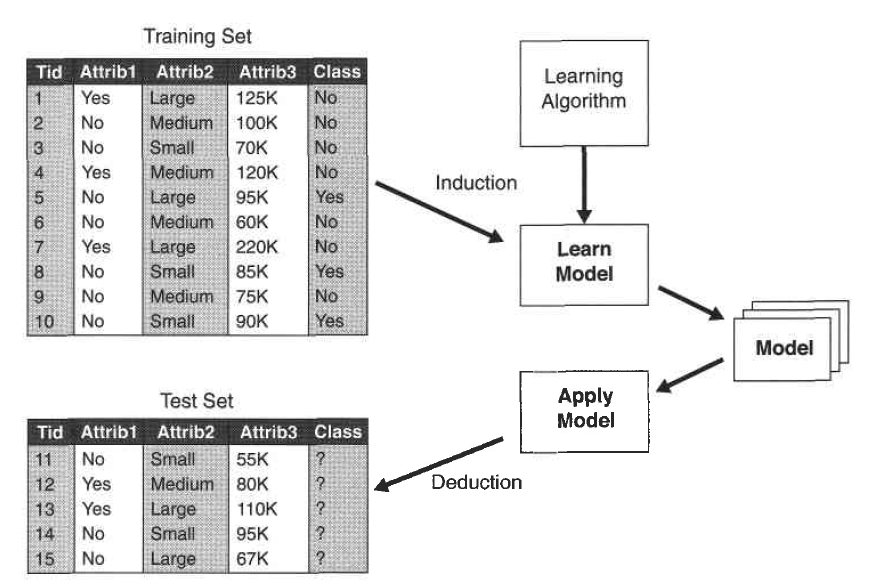
\includegraphics[scale=0.4]{bab2/classificationmodel}  
	\caption{Proses Klasifikasi} 
	\label{fig:classificationprocess}
\end{figure} 

Gambar \ref{fig:classificationprocess} menunjukkan sebuah proses dalam melakukan \textit{classification}. \textit{Classifier} / \textit{classification technique} adalah sebuah cara untuk membuat model dari \textit{input data set}. Pada awalnya, \textit{dataset} dapat dibagi menjadi 2 bagian yaitu \textit{training set} dan \textit{test set}. Terdapat \textit{training set} yaitu kumpulan data / \textit{record} yang sudah memiliki label data akan di\textit{train} modelnya dengan menggunakan algoritma \textit{classification}. Model yang sudah dibuat akan digunakan untuk memrediksi nilai label dari data yang ingin diprediksi yaitu \textit{test set} untuk diuji keakuratannya. Hasil nilai label yang sudah diprediksi dapat dinilai dengan cara membandingkan hasil prediksi label dengan label asli pada \textit{test set}.


Dalam memanfaatkan \textit{classification} untuk memrediksi nilai label, terdapat beberapa algoritma yang dapat dimanfaatkan untuk melakukan \textit{classification} yaitu \textit{Decision Tree} ,\textit{k Nearest Neighbors} (kNN), dan \textit{Naive Bayes Classifier}.

\subsubsection{Decision Tree} 
\textit{Decision tree} adalah teknik \textit{classifier} dapat digunakan untuk menentukan label data pada \textit{test set}. \textit{Decision tree} akan membentuk sebuah pohon keputusan berdasarkan atribut prediktor yang akan digunakan untuk membuat model. Pohon keputusan yang dihasilkan akan menjadi aturan bagaimana menentukan label dari \textit{data set}. Membuat \textit{Decision tree} akan memanfaatkan \textit{training set} untuk menentukan berdasarkan apa pohon dapat di\textit{split}. 

Struktur sebuah pohon keputusan memiliki 3 \textit{node} yaitu : 
\begin{itemize}
\item \textbf{\textit{Root node}} : tidak memiliki \textit{incoming edge} dan tidak atau banyak \textit{edges}
\item \textbf{\textit{Internal nodes}} : memiliki satu \textit{incoming edge} dan banyak \textit{outgoing edges} 
\item \textbf{\textit{Leaf / terminal nodes}} memiliki satu \textit{incoming edge} dan tidak ada \textit{outgoing edges}
\end{itemize}
\pagebreak
\begin{figure}[h!]
	\centering  
	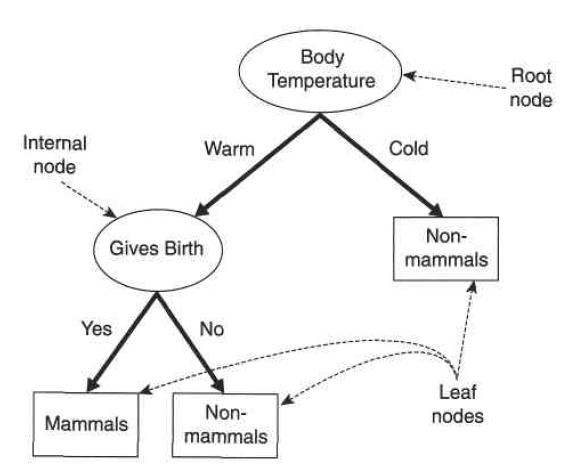
\includegraphics[scale=0.4]{bab2/decisiontreeexample}   
	\caption{Ilustrasi Decision Tree}
	\label{fig:decisiontreeexample} 
\end{figure} 

Gambar \ref{fig:decisiontreeexample} menunjukkan sebuah contoh bagaimana penerapan pohon keputusan pada sebuah \textit{dataset} binatang. Tujuan dari pohon keputusan adalah untuk menentukan aturan apakah sebuah binatang termasuk \textit{mammals} atau \textit{non-mammals}. Atribut prediktor yang terdapat ada \textit{root node} dan \textit{internal node}seperti \textit{Body temperature} dan \textit{Given Birth} digunakan untuk memecah \textit{data} agar dapat menentukan label. 


Teknik ini dapat menghasilkan berbagai pohon keputusan berdasarkan attribut yang dipilih sebagai atribut pembagi. Untuk menghasilkan \textit{model} yang akurat, dibutuhkan cara untuk menentukan atribut yang dapat membagi pohon. Cara memilih atribut adalah dengan mengukur tingkat \textit{impurity} / ketidakmurnian dari \textit{node}. Tujuan dari pembuatan pohon keputusan ini adalah untuk membuat semua \textit{node} \textit{pure} / murni. Sebuah \textit{node} dapat dikatakan murni jika sudah memiliki label data. 

\textit{Entropy} adalah ukuran \textit{randomness} / ketidakpastian sebuah data. Semakin rendah nilai \textit{entropy}, maka semakin murni \textit{node} tersebut. Rumus dari entropi adalah yaitu :

\begin{equation}
Entropy(t) = - \sum_{i=0}^{c-1} p(i|t)\log_2 (i|t)
\label{eqref:entropi}
\end{equation}

Berdasarkan uraian rumus \eqref{eqref:entropi} , perhitungan entropi merupakan penjumlahan peluang tiap kelas  \textit{i} terhadap semua jumlah data \textit{t}. Untuk menentukan atribut mana yang dapat digunakan sebagai pemecah, kita butuh untuk membandingkan tingkat ketdakmurnian \textit{parent node} (sebelum dipecah) dengan  tingkat ketidakmurnian dari \textit{child node} (setelah dipecah).  \textit{\textbf{Information Gain}} ($\Delta$ info) adalah sebuah kriteria yang dapat digunakan untuk menentukan atribut pembagi dalam pembentukan pohon. Rumus dari \textit{information gain}  yaitu : 

\begin{equation}
  \Delta info = I(parent) - \sum_{j=1}^{k} \frac{N(vj)}{N}I(jv)
  \label{eqref:information gain}
\end{equation}

rumus \eqref{eqref:information gain} \textit{I} adalah nilai ketidakmurnian yang dapat diperoleh menggunakan \textit{entropy}. N adalah total observasi data / jumlah \textit{record} dari \textit{parent node}, \textit{k} adalah jumlah nilai dari suatu atribut, dan \textit{vj} adalah jumlah \textit{record} pada nilai atribut j. \textit{Decision} tree akan memilih atribut prediktor mana dengan memilih nilai $\Delta$ (info) yang maksimum.

\subsubsection{K-Nearest Neighbor Classifiers}
 \textit{K-Nearest Neighbor} adalah algoritma \textit{classification} untuk menentukan label sebuah data. \textit{K-Nearest Neighbor} akan menentukan label data baru berdasarkan \textit{dataset} yang sudah memiliki label pada \textit{training set}. Menentukan label untuk data baru dapat ditentukan dengan mencari  \textit{training data} yang terdekat dengan data baru. Label pada \textit{k}-jarak terdekat menjadi label bagi data baru. Setiap data pada \textit{dataset} dapat dianalogikan sebagai titik yang akan dibandingkan jaraknya. Menghitung jarak antara titik data baru dan setiap titik pada \textit{dataset} dapat menggunakan \textit{euclidean distance}. Menghitung \textit{Euclidean distance} adalah dengan rumus : 

\begin{equation}
	dist(X,Y) = \sqrt[]{\sum_{n}^{i=1}(xi-yi)^2}
	\label{eqref:euclideandistanceknn}
\end{equation}

Uraian rumus \eqref{eqref:euclideandistanceknn} di atas merupakan cara menghitung jarak antara titik baru dengan suatu titik pada \textit{training set}. X merupakan data baru dan Y merupakan suatu titik pada \textit{training set}. Xi merupakan setiap atribut variabel pada data baru dan Yi merupakan setiap atribut variabel pada titik \textit{training set}. Algoritma \textit{k-Nearest Neighbor} akan menghitung \textit{euclidean distance} sebanyak N yaitu jumlah \textit{row} pada \textit{training set} untuk membandingkan jarak data baru dengan setiap data pada \textit{training set}. Semakin kecil nilai \textit{euclidean distance} maka 2 titik yang dibandingkan akan semakin dekat. \\

Selain \textit{euclidean distance}, \textit{Cosine Similarity} juga dapat digunakan untuk mengukur kemiripan 2 vektor. Menghitung \textit{Cosine Distance} adalah dengan rumus : 

\begin{equation}
   sim(x,y)  = \frac{x \cdot y}{||x|| ||y||}
   \label{eqref:cosinesimilarity}
\end{equation}

Uraian rumus \eqref{eqref:cosinesimilarity} adalah cara lain untuk mengukur seberapa dekat / mirip 2 vektor. $x \cdot y$ dibagian atas adalah merupakan \textit{Dot Product} dari 2 vektor. \textit{Dot Product} dapat dihitung dengan cara mengalikan tiap elemen diurutan yang sama lalu dijumlahkan. Bagian bawah merupakan perkalian dari panjang vektor x dan y. Rumus panjang vektor adalah berdasarkan rumus \eqref{eqref:vectorlength} dibawah yaitu penjumlahan setiap elemen vektor x yang dikuadratkan lalu diakar :

\begin{equation}
  \vec{x} = \sqrt[]{\sum{i}^{n} (x_i)^2}
  \label{eqref:vectorlength}
\end{equation}


Menggunakan \textit{euclidean distance} dapat diterapkan untuk atribut dengan tipe data numerik. Tetapi, untuk atribut nominal seperti jenis warna (biru,merah, hijau dan lain-lain) membutuhkan mekanisme berbeda untuk menentukan jarak terdekat. Menentukan angkanya adalah jika nilai atribut data baru sama dengan data pada \textit{training set} maka jaraknya adalah 0. Jika nilai atirbut data baru tidak sama dengan sebuah data pada \textit{training set}, maka jaraknya adalah 1. 

Tahap pertama dalam mencari label untuk data baru menggunakan \textit{k-Nearest Neighbor} adalah  dengan menentukan k tetangga terdekat. Cara menentukan k terbaik adalah dengan mencoba menghitung jarak pada setiap k. K terbaik dapat ditentukan dengan mencari akurasi tertinggi dari setiap percobaan k.

 
\subsubsection{Evaluasi Classification} 
Cara yang dapat digunakan untuk melakukan evaluasi terhadap model yang sudah dibuat adalah dengan menghitung jumlah perbandingan data yang benar dan salah. \textit{Accuracy} adalah sebuah metode \textit{performance metric} yang dapat digunakan untuk menghitung performa model. Cara menghitung akurasi yaitu : 

\begin{displaymath}
    Accuracy  = \frac{Jumlah prediksi yang benar}{Jumlah semua prediksi}
\end{displaymath} 

\textit{Error rate} adalah cara lain yang dapat digunakan sebagai menilai performa model berdasarkan nilai \textit{error} yang dihasilkan. Cara menghitung \textit{error rate} adalah sebagai berikut : 

\begin{displaymath}
 Error rate = \frac{Jumlah prediksi yang salah}{Jumlah semua prediksi}
\end{displaymath}

%	RKS: MACHINE LEARNING - > CLUSTERING 
\subsection{Clustering}
\textit{Clustering} merupakan teknik \textit{unsupervised learning}. \textit{Clustering} dapat mengelompokkan tiap data objek pada \textit{dataset} menjadi beberapa kelompok. \textit{Clustering} mengelompokkan data objek yang memiliki kemiripan menjadi satu kelompok dan data objek yang tidak memiliki kemiripan menjadi kelompok yang berbeda. Kemiripan dan ketidakmiripan dari data objek dapat ditentukan menggunakan atribut prediktor pada \textit{dataset}. Ukuran yang dapat ditentukan untuk kemiripan tiap data objek adalah berdasarkan perhitungan jarak. Terdapat beberapa metode \textit{clustering} yaitu : 

\begin{itemize}

\item \textbf{Partitioning methods} : metode \textit{clustering} dengan membuat k partisi dimana jumlah partisi (k) <= N (jumlah data objek). Tiap partisi harus minimal berisi satu data objek. Contoh algoritma \textit{partitioning} adalah \textit{k-Means} 

\item \textbf{Hierarchical methods} : metode \textit{clustering} dengan cara melakukan proses dekomposisi menjadi hirarki. Hirarki yang dihasilkan adalah tingkatan jumlah kelompok yang dihasilkan. Terdapat dua jenis \textit{Hierarchical methods} yaitu \textit{agglomerative} dan \textit{divisive}. \textit{Agglomerative} menerapkan \textit{bottom-up approach}. \textit{Agglomerative} berawal dari tiap data objek pada \textit{dataset} menjadi data yang terpisah. Masing-masing data objek digabung satu per satu sehingga membentuk satu kelompok yang besar. \textit{Divisive} menerapkan \textit{top-bottom approach} yaitu setiap data objek yang dijadikan satu kelompok besar. Setiap iterasi akan dibagi menjadi kelompok-kelompok kecil sampai tiap data objek merupakan kelompok yang terpisah.

\item \textbf{Density-based methods} : metode \textit{clustering} dengan cara membagi kumpulan data objek menjadi bentuk kelompok yang lebih kompleks. Contoh algoritma \textit{density} adalah \textit{Density Based Spatial Clustering} (DBSCAN). Cara kerjanya adalah setiap data objek yang merupakan titik secara acak diambil  untuk ditentukan jenisnya. Suatu titik merupakan \textit{core points} jika masih memiliki tetangga yang jaraknya lebih kecil dari epsilon. Jika tidak terdapat titik tetangga terdekat, titik dijadikan sebuah \textit{border points}. Setelah itu berpindah ke titik tetangga \textit{core points} terdekat lalu diulangi lagi sampai semua menjadi mempunyai \textit{cluster} atau \textit{outlier}
\end{itemize}

\subsubsection{K-Means}
\textit{K-Means} adalah algoritma \textit{clustering} jenis \textit{partitioning}. Algoritma ini mengelompokkan data objek dengan memaksimalkan kemiripan. Ukuran kemiripan antar data objek dapat diukur menggunakan jarak. Jumlah kelompok akan ditentukan berdasarkan nilai k yang ditentukan. Setelah nilai k telah ditentukan, maka akan dibuat data objek secara \textit{random} atau mengambil salah satu data pada \textit{data set} yang disebut sebagai \textit{centroid}. \textit{Centroid} merupakan nilai tengah yang merepresentasikan tiap \textit{cluster}. Tiap data objek akan dihitung jaraknya dengan setiap \textit{centroid} yang diinisialisasi. Data objek akan dimasukkan ke kelompok \textit{cluster} yang memiliki jarak terkecil dengan \textit{centroid}. Jarak data objek dengan centroid dapat dihitung dengan menggunakan \textit{euclidean distance}: 

\begin{equation}
	dist(X,Y) = \sqrt[]{\sum_{n}^{i=1}(xi-yi)^2}
	\label{eqref:euclideandistance}
\end{equation}

Persamaan \eqref{eqref:euclideandistance} menghitung jarak antara 2 data objek. X adalah data objek pertama dan Y adalah data objek kedua. $\sum_{}^{}$ adalah melakukan iterasi dan penjumlahan setap atribut. Setiap atribut masing-masing data objek akan dikurang lalu dipangkatkan. Hasil perpangkatan selisih setiap atribut akan diakarpangkat dua sehingga menjadi jarak dari kedua data objek

Langkah-langkah dalam melakukan \textit{k-Means clustering} adalah : 
\begin{enumerate}
\item Tentukan jumlah K (jumlah \textit{cluster} / kelompok)
\item Untuk tiap \textit{cluster}, buat satu data objek sebagai titik tengah yang disebut sebagai \textit{centroid}. Inisialisasi \textit{centroid} dapat ditentukan dengan \textit{random} / mengambil salah satu titik dari \textit{data objek} 
\item Untuk setiap data objek, hitung jarak menggunakan \textit{euclidean distance} dengan setiap \textit{centroid}. Data objek akan masuk ke kelompok yang memiliki \textit{centroid} dengan jarak terpendek
\item Atur ulang posisi \textit{centroid} dengan menghitung rata-rata tiap atribut yang termasuk dalam \textit{cluster} 
\item Ulangi tahap tiga sampai tiap data objek tidak mengalami perubahan dalam menetapkan \textit{cluster}
\end{enumerate}



\subsubsection{Agglomerative Nesting (AGNES)}
\textit{Agglomerative clustering} adalah algoritma \textit{clustering} jenis \textit{hierarchical}. Algoritma ini merupakan metode \textit{bottom-up} yaitu setiap data objek sebagai masing-masing \textit{cluster}. Secara iteratif menghitung jarak tiap data objek. Dua data objek dengan jarak terkecil akan digabung menjadi sebuah \textit{cluster}. Proses ini diulangi sampai semua data objek tergabung menjadi satu \textit{cluster}. Jarak tiap titik dapat dihitung menggunakan \textit{euclidean distance} pada Persamaan (\ref{eqref:euclideandistance}) atau menggunakan \textit{cosine distance} pada Persamaan (\ref{eqref:cosinesimilarity}). 


\pagebreak

\subsubsection{Evaluasi Clustering}
Pengelompokan data dapat dilakukan menggunakan \textit{clustering}, tetapi pengaruh pemilihan jumlah K / berapa kelompok pada algoritma dan metrik jarak yang digunakan dapat berpengaruh terhadap seberapa baik / seberapa mirip anggota dari \textit{cluster} yang dihasilkan. Terdapat beberapa cara untuk mengukur apakah \textit{clustering} yang dilakukan sesuai kebutuhan / akurat. Terdapat 2 cara dalam mengukur \textit{clustering} yaitu \textit{intracluster} dan \textit{silhouette plot}

\paragraph{Intracluster} \mbox{}\\
\textit{Intracluster} adalah nilai yang merepresentasikan apakah sebuah \textit{cluster} dikelompokkan dengan baik. \textit{Cluster} yang baik adalah \textit{cluster} yang jarak tiap anggotanya dekat / mirip. Cara menghitung \textit{intracluster} sebuah titik adalah dengan menghitung jarak titik tersebut dengan titik representatif dari \textit{cluster}. Titik representatif adalah \textit{centroid} yaitu rata-rata dari tiap anggota pada \textit{cluster} yang sama. Berikut adalah rumus cara menghitung \textit{intracluster} yaitu :

\begin{equation}
intracluster  = \frac{\sum_{i=1}^{n}(Jarak Titik (i) dengan Centroid)}{Jumlah Anggota pada Cluster tersebut}
\label{eqref:rumusintracluster}
\end{equation}

Berdasarkan persamaan \eqref{eqref:rumusintracluster} di atas, untuk menghitung \textit{intracluster} sebuah kelompok adalah dengan menghitung rata-rata jarak tiap titik yang merupakan kelompok tersebut dengan \textit{centroid}. Perhitungan jarak dapat menggunakan \textit{euclidean distance} atau \textit{cosine distance}.

\paragraph{Silhouette Plot} \mbox{}\\
\textit{Silhouette Plot} merupakan teknik yang digunakan untuk mengukur kualitas sebuah \textit{cluster}. Teknik ini menggabungkan kualitas internal (Intracluster) dan eksternal (Intercluster). Menghitung \textit{silhouette plot} adalah dengan rumus berikut yaitu : 

\begin{equation}
  S(i) = \frac{(b(i)-a(i))}{max(a(i),b(i))}
\label{eqref:silhouetteplot}
\end{equation}

Persamaan \eqref{eqref:silhouetteplot} di atas adalah cara menghitung kualitas sebuah titik pada \textit{cluster}. $S(i)$ adalah nilai \textit{silhouette} pada sebuah titik pada \textit{cluster}. $b(i)$ adalah nilai rata-rata jarak titik tersebut dengan titik lain dalam sebuah \textit{cluster} yang sama. $a(i)$ adalah nilai rata-rata jarak titik tersebut dengan titik tetangga. Titik tetangga adalah tiap titik terdekat dengan titik yang sedang dihitung tetapi masing-masing berasal dari \textit{cluster} yang berbeda. \\

Untuk mendapatkan kualitas \textit{cluster} secara keseluruhan adalah dengan menghitung rata-rata dari nilai \textit{silhouette plot} dari tiap titik dataset. Nilai \textit{silhouette plot} bisa berada diantara $0.0$ sampai $1.0$.  Semakin besar nilai \textit{cluster} maka semakin baik \textit{clustering} yang dilakukan.

\section{Data Visualization \cite{han2012mining} } 
Visualisasi data adalah suatu metode untuk merepresentasikan data. Visualisasi data menggunakan dengan jumlah yang banyak untuk ditampilkan secara grafis. Visualisasi data akan membantu \textit{user} untuk membaca data lebih mudah. Dengan visualisasi, maka kita juga akan mendapatkan informasi mengenai hubungan antara data. Visualisasi data akan membantu meringkaskan data dan memberikan pengetahuan baru. 
		
Penggunaan visualisasi data dapat digunakan pada saat \textit{data preprocessing} maupun setelahnya. Pada tahap \textit{data preprocessing}, visualisasi data dapat dimanfaatkan untuk membantu proses memeriksa data untuk memastikan kebersihannya. Visualisasi data tidak hanya dilakukan sekali tetapi membutuhkan beberapa kali visualisasi untuk membantu menganalisis tren dari perubahan data itu sendiri. 
		
 Visualisasi data dapat dibedakan berdasarkan tipe data yang dianalisis, jumlah atribut yang digunakan, dan bentuk data yang dibutuhkan. Terdapat beberapa teknik yang dilakukan untuk melakukan visualisasi data yaitu \textit{Box plot}, \textit{Histogram}, \textit{Scatter plot} dan \textit{Pie chart} \\
 
\subsection{Boxplot}	
\textit{Boxplot} adalah teknik \textit{data visualization} yang dapat digunakan untuk menampilkan persebaran nilai satu atribut. Masukan data dari grafik ini adalah kumpulan atribut numerik. Teknik ini dapat membantu memberikan informasi mengenai nilai-nilai yang dapat digunakan untuk analisis data. Suatu \textit{Boxplot} akan menampilkan rata-rata(\textit{mean}), median (Q2), nilai maksimum, nilai minimum, kuartil bawah(Q1)dan kuartil atas(Q3). Berikut adalah  contoh \textit{box plot} yang dihasilkan berdasarkan \textit{dataset} iris pada kolom \textit{sepal length} yaitu :
			
\begin{figure}[h!]
	\centering  
	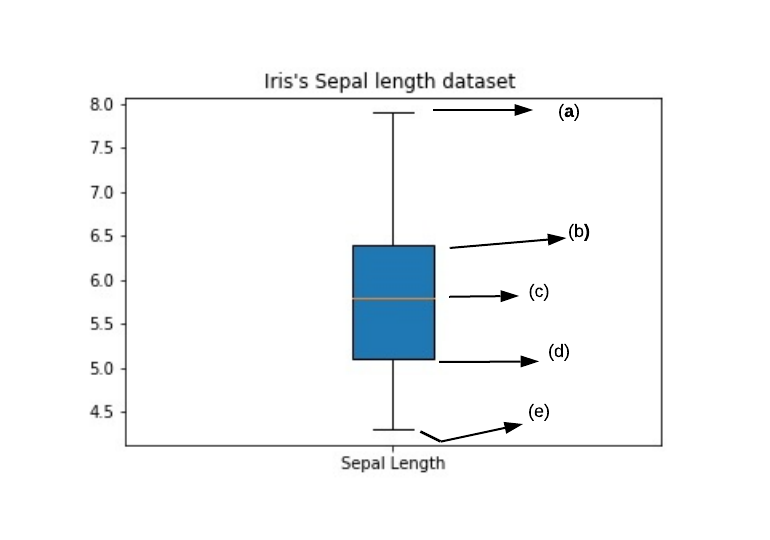
\includegraphics[scale=0.7]{bab2/boxplot}   
	\caption{Boxplot dataset iris}
	\label{fig:boxplot} 
\end{figure} 
 Gambar \ref{fig:boxplot} menunjukkan kesimpulan informasi dari persebaran \textit{dataset} iris pada kolom \textit{sepal length}. Berikut adalah deskripsi dari tiap huruf : 
	 	\begin{itemize}
	 	\item \textbf{(a)} nilai maksimum 
	 	\item \textbf{(b)} kuartil atas (Q3) 
	 	\item \textbf{(c)} median (Q2) 
	 	\item \textbf{(d)} kuartil bawah (Q1)
	 	\item \textbf{(e)} nilai minimum 
	 	\end{itemize}
\pagebreak 	

\subsection{Histogram} 
 \textit{Histogram} adalah teknik \textit{data visualization} yang digunakan untuk melihat persebaran data suatu atribut. Masukan dari  Data yang ditampilkan akan dibagi dalam sebuah \textit{bin} / interval kelas. Teknik ini akan mengelompokkan jumlah \textit{data object} berdasarkan nilai interval yang ditentukan dan sudah terurut. Berikut adalah contoh \textit{histogram} dari \textit{dataset iris sepal width} yaitu :
	 	
	 	   	
\begin{figure}[h!]
	\centering  
	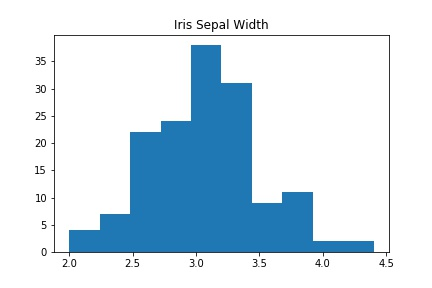
\includegraphics[scale=0.7]{bab2/histogramiris}   
	\caption{Histogram dataset iris}
	\label{fig:histogram} 
\end{figure} 
	
	
 Histogram yang ditampilkan pada gambar diatas adalah berdasarkan \textit{dataset iris}. \textit{Dataset iris} merupakan data spesies bunga yang paling sering digunakan. Berdasarkan gambar \ref{fig:histogram}, histogram satu variabel akan menunjukkan grafik dengan koordinat 2 dimensi yaitu koordinat x dan y. Nilai pada koordinat x menunjukkan tiap interval kelas. Nilai pada koordinat y menunjukkan frekuensi tiap interval data. Tiap batang pada histogram menampilkan tiap interval kelas. Tinggi batang menunjukkan frekuensi pada tiap kelas.
		
 Pada contoh gambar \ref{fig:histogram}, terdapat 10 \textit{bins} / batang yang masing-masingnya memiliki rentang sekitar nilai interval 0,25. Pada \textit{bin} pertama, terdapat jarak nilai dari 2.0 sampai kurang lebih 2,25. Aturan juga diterapkan pada \textit{bin} 2 sampai 10 yaitu menyerupai  \textit{bin} pertama. \\ 
 
 
\subsection{Scatter Plot} 
 \textit{Scatter plot} adalah teknik \textit{data visualization} yang dapat digunakan untuk melihat korelasi / keterhubungan antara 2 variabel data. \textit{Scatter plot} akan menggambarkan atribut prediktor (sebab) pada koordinat X dan menggambarkan atribut respon (akibat) pada koordinat Y. Hasil \textit{scatter plot} akan memberi penjelasan apakah atribut prediktor memiliki hubungan dengan atribut respon. Terdapat beberapa jenis \textit{Scatter plot} berdasarkan hasil korelasinya. Terdapat \textit{Scatter plot} yang memiliki korelasi positif, korelasi negatif dan tidak memiliki korelasi. Berikut adalah contoh gambar \textit{scatter plot} yaitu
 
\pagebreak
		\begin{figure}[h!]
		\centering  
		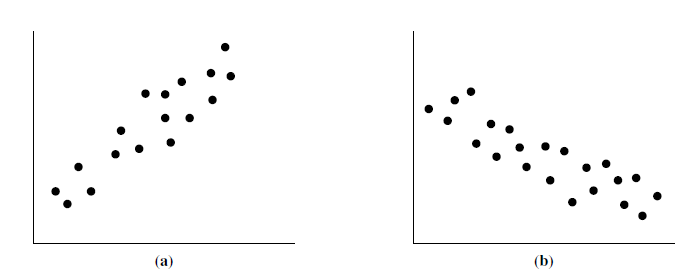
\includegraphics[scale=0.7]{bab2/scatterplotcorrelation}   
		\caption{Scatter plot dengan korelasi positif (a) dan negatif (b)}
		\label{fig:scatterplotcorrelation} 
	\end{figure} 
	
	\begin{figure}[h!]
		\centering  
		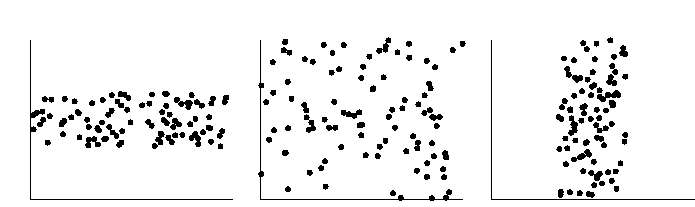
\includegraphics[scale=0.7]{bab2/scatterplotwithoutcorrelation}   
		\caption{Scatter plot tanpa korelasi}
		\label{fig:scatterplotwithoutcorrelation} 
	\end{figure} 
	
Berdasarkan Gambar \ref{fig:scatterplotcorrelation}, \textit{scatter plot} dengan korelasi terbentuk jika perubahan atribut pada koordinat X memengaruhi koordinat Y. Korelasi positif terjadi ketika semakin meningkatnya nilai pada koordinat X, maka koordinat Y akan meningkat juga. Korelasi negatif terjadi ketika perubahan koordinat X akan membuat nilai pada koordinat Y berubah berbanding terbalik. Gambar \ref{fig:scatterplotwithoutcorrelation} menggambarkan atribut koordinat X dan koordinat Y tidak memiliki korelasi.  

\subsection{Pie Chart}
\textit{Pie Chart} adalah teknik \textit{data visualization} untuk melihat frekuensi persebaran \textit{categorial data}. \textit{Pie chart} menggunakan bentuk lingkaran sebagai keseluruhan semua kumpulan data. Masing-masing potongan bagian pada \textit{pie chart} merupakan presentase banyak masing-masing nilai kategori. Berikut adalah gambaran \textit{pie chart} menggunakan \textit{dataset iris}. 
	
	\begin{figure}[H]
		\centering  
		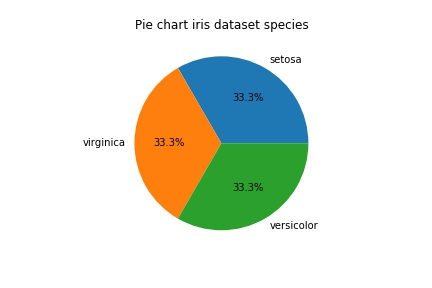
\includegraphics[scale=0.7]{bab2/piechart}   
		\caption{Pie chart dataset iris}
		\label{fig:piechart} 
	\end{figure}
	
Berdasarkan Gambar \ref{fig:piechart}, data yang digunakan untuk divisualisasikan adalah \textit atribut {species dataset iris}. Pada \textit{dataset} terdapat atribut \textit{species} yang memiliki kemungkinan nilai yaitu \textit{setosa, virginica, versicolor}. Tiap warna pada \textit{pie chart} merepresentasikan masing-masing kategori \textit{species}. Jumlah data pada atribut \textit{species} adalah 150, jumlah masing-masing \textit{species} adalah 50 sehingga presentasenya sama.

\section{One Hot Encoding \cite{tan_steinbach_karpatne_kumar_2020}}
\label{chap:teori_onehotencoding}
\textit{One hot encoding} adalah metode yang dapat digunakan untuk mengubah data kategorial menjadi numerik. Nilai label yang dimiliki tipe data kategorial tidak bisa dihitung / kuantifikasi jika data tersebut digunakan pada \textit{machine learning}. \textit{Machine learning} sering memanfaatkan perhitungan jarak pada data numerik untuk menghitung kemiripan 2 data objek. \textit{One hot encoding} tidak dapat digunakan pada data ordinal. Data ordinal yaitu tipe data kategorial yang tiap nilainya memiliki sifat keterurutan. \textit{One hot encoding} cocok untuk nilai kategorial yang tidak memiliki unsur keterurutan / sederajat.


\section{Web Scraping  \cite{manning_raghavan_schutze_2018}}
\textit{Web Scraping} adalah metode untuk mengambil data dari sebuah \textit{web page}. \textit{Scraping} dapat dilakukan untuk mengambil elemen yang terdapat pada halaman web. \textit{Scraping} dapat dilakukan dengan \textit{web scraper} dan \textit{web crawler}. \textit{Web scraping} akan membantu dalam mengumpulkan data yang banyak dari kumpulan \textit{website}. Dasar perintah dalam \textit{scraping} adalah :

\begin{enumerate}
\item Mengambil URL sebuah halaman web
\item Melakukan Parsing pada sebuah halaman 
\item Melakukan ekstraksi data URL 
\item Memasukan URL pada \textit{queue}
\end{enumerate}

Berdasarkan tahap yang dijelaskan sebelumnya, proses \textit{web scraping} ini akan diulang selama masih ada halaman / URL pada \textit{queue} yang terhubung dari URL sebelumnya dan mengambil data pada halaman.

\section{Istilah Dalam Bisnis Film}
Terdapat beberapa istilah yang perlu dipahami mengenai bisnis industri film yaitu :

\begin{itemize}
\item Budget : biaya yang dikeluarkan untuk memproduksi film 
\item Revenue / pendapatan kotor : pemasukan yang diterima dari hasil penjualan film 
\item Profit / pendapatan bersih : hasil pengurangan \textit{revenue} dan \textit{budget}

\item \textit{Return Of Investment (ROI)} :  rasio yang mengukur efisiensi sebuah investasi dengan membandingkan \textit{profit} dengan \textit{budget} yang dikeluarkan
\end{itemize}

%
%\section{Skripsi}
%\label{sec:skripsi} 
% 
%Rencananya akan diisi dengan penjelasan umum mengenai buku skripsi.
%
%\dtext{11-12} 
%
%\section{\LaTeX}
%\label{sec:latex}
%
%Mengapa menggunakan \LaTeX{} untuk buku skripsi dan apa keunggulan/kerugiannya bagi mahasiswa dan pembuat template. 
%
%\dtext{13-14}
%
%
%\section{Template Skripsi FTIS UNPAR}
%\label{sec:template}
% 
%Akan dipaparkan bagaimana menggunakan template ini, termasuk petunjuk singkat membuat referensi, gambar dan tabel.
%Juga hal-hal lain yang belum terpikir sampai saat ini. 
% 
%\dtext{15-16}
%
%\subsection{Tabel}  
%Berikut adalah contoh pembuatan tabel. 
%Penempatan tabel dan gambar secara umum diatur secara otomatis oleh \LaTeX{}, perhatikan contoh di file bab2.tex untuk melihat bagaimana cara memaksa tabel ditempatkan sesuai keinginan kita.
%
%Perhatikan bawa berbeda dengan penempatan judul gambar gambar, keterangan tabel harus diletakkan di atas tabel!!
%Lihat Tabel~\ref{tab:contoh1} berikut ini:
%
%\begin{table}[H] %atau h saja untuk "kira kira di sini"
%	\centering 
%	\caption{Tabel contoh}
%	\label{tab:contoh1}
%	\begin{tabular}{cccc}
%		\toprule
%		& $v_{start}$ & $\mathcal{S}_{1}$ & $v_{end}$\\
%
%		\midrule
%		$\tau_{1}$ & 1 & 12& 20\\
%		$\tau_{2}$ & 1 &  & 20\\
%		$\tau_{3}$ & 1 & 9 & 20\\
%		$\tau_{4}$ & 1 &  & 20\\
%
%		\bottomrule
%		
%	\end{tabular} 
%\end{table}
%Tabel~\ref{tab:cthwarna1} dan Tabel~\ref{tab:cthwarna2} berikut ini adalah tabel dengan sel yang berwarna dan ada dua tabel yang bersebelahan. 
%\begin{table}[H]
%	\begin{minipage}[c]{0.49\linewidth}
%		\centering
%		\caption{Tabel bewarna(1)}
%		\label{tab:cthwarna1}
%		\begin{tabular}{ccccc}
%			\toprule
%			 & $v_{start}$ & $\mathcal{S}_{2}$ & $\mathcal{S}_{1}$ & $v_{end}$\\
%			
%			\midrule
%			$\tau_{1}$ & 1 & 5 \cellcolor{green}& 12& 20\\
%			$\tau_{2}$ & 1 & 8 \cellcolor{green}& & 20\\
%			$\tau_{3}$ & 1 & 2/8/17 \cellcolor{green}& 9 & 20\\
%			$\tau_{4}$ & 1 & \cellcolor{red}& & 20\\
%			
%			\bottomrule
%
%		\end{tabular}
%	\end{minipage}
%	\begin{minipage}[c]{0.49\linewidth}
%		
%		\centering 
%		\caption{Tabel bewarna(2)}
%		\label{tab:cthwarna2}
%		\begin{tabular}{ccccc}
%			\toprule
%			 & $v_{start}$ & $\mathcal{S}_{1}$ & $\mathcal{S}_{2}$ & $v_{end}$\\
%			
%			\midrule
%			$\tau_{1}$ & 1 & 12& 5 \cellcolor{red} &20\\
%			$\tau_{2}$ & 1 &  &  8 \cellcolor{green} &20\\
%			$\tau_{3}$ & 1 & 9 & 2/8/17 \cellcolor{green} &20\\
%			$\tau_{4}$ & 1 &   & \cellcolor{red} &20\\
%			
%			\bottomrule
%		
%		\end{tabular}
%	\end{minipage}
%\end{table}
%
% 
%\subsection{Kutipan}
%\label{subs:kutipan} 
%Berikut contoh kutipan dari berbagai sumber, untuk keterangan lebih lengkap, silahkan membaca file referensi.bib yang disediakan juga di template ini.
%Contoh kutipan:
%\begin{itemize}
%	\item Buku:~\cite{berg:08:compgeom} 
%	\item Bab dalam buku:~\cite{kreveld:04:GIS}
%	\item Artikel dari Jurnal:~\cite{buchin:13:median}
%	\item Artikel dari prosiding seminar/konferensi:~\cite{kreveld:11:median}
%	\item Skripsi/Thesis/Disertasi:~\cite{lionov:02:animasi}~\cite{wiratma:10:following}~\cite{wiratma:22:later}
%	\item Technical/Scientific Report:~\cite{kreveld:07:watertight}
%	\item RFC (Request For Comments):~\cite{RFC1654}
%	\item Technical Documentation/Technical Manual:~\cite{Z.500}~\cite{unicode:16:stdv9}~\cite{google:16:and7}
%	\item Paten:~\cite{webb:12:comm}
%	\item Tidak dipublikasikan:~\cite{wiratma:09:median}~\cite{lionov:11:cpoly}
%	\item Laman web:~\cite{erickson:03:cgmodel}  
%	\item Lain-lain:~\cite{agung:12:tango}
%\end{itemize}    
%  
%\subsection{Gambar}
%
%Pada hampir semua editor, penempatan gambar di dalam dokumen \LaTeX{} tidak dapat dilakukan melalui proses {\it drag and drop}.
%Perhatikan contoh pada file bab2.tex untuk melihat bagaimana cara menempatkan gambar.
%Beberapa hal yang harus diperhatikan pada saat menempatkan gambar:
%\begin{itemize}
%	\item Setiap gambar {\bf harus} diacu di dalam teks (gunakan {\it field} {\sc label})
%	\item {\it Field} {\sc caption} digunakan untuk teks pengantar pada gambar. Terdapat dua bagian yaitu yang ada di antara tanda $[$ dan $]$ dan yang ada di antara tanda $\{$ dan $\}$. Yang pertama akan muncul di Daftar Gambar, sedangkan yang kedua akan muncul di teks pengantar gambar. Untuk skripsi ini, samakan isi keduanya.
%	\item Jenis file yang dapat digunakan sebagai gambar cukup banyak, tetapi yang paling populer adalah tipe {\sc png} (lihat Gambar~\ref{fig:ularpng}), tipe {\sc jpg} (Gambar~\ref{fig:ularjpg}) dan tipe {\sc pdf} (Gambar~\ref{fig:ularpdf})
%	\item Besarnya gambar dapat diatur dengan {\it field} {\sc scale}.
%	\item Penempatan gambar diatur menggunakan {\it placement specifier} (di antara tanda  $[$ dan $]$ setelah deklarasi gambar.
%	Yang umum digunakan adalah {\bf H} untuk menempatkan gambar {\bf sesuai} penempatannya di file .tex atau  {\bf h} yang berarti "kira-kira" di sini. \\
%	Jika tidak menggunakan {\it placement specifier}, \LaTeX{} akan menempatkan gambar secara otomatis untuk menghindari bagian kosong pada dokumen anda.
%	Walaupun cara ini sangat mudah, hindarkan terjadinya penempatan dua gambar secara berurutan. 	
%	\begin{itemize}
%		\item Gambar~\ref{fig:ularpng} ditempatkan di bagian atas halaman, walaupun penempatannya dilakukan setelah penulisan 3 paragraf setelah penjelasan ini.
%		\item Gambar~\ref{fig:ularjpg} dengan skala 0.5 ditempatkan di antara dua buah paragraf. Perhatikan penulisannya di dalam file bab2.tex!
%		\item Gambar~\ref{fig:ularpdf} ditempatkan menggunakan {\it specifier} {\bf h}.
%	\end{itemize}
%\end{itemize}
% 
%\dtext{17-18}
%\begin{figure} 
%	\centering  
%	\includegraphics[scale=1]{ular-png}  
%	\caption[Gambar {\it Serpentes} dalam format png]{Gambar {\it Serpentes} dalam format png} 
%	\label{fig:ularpng} 
%\end{figure} 
%
%\dtext{19-20}
%\begin{figure}[H]
%	\centering  
%	\includegraphics[scale=0.5]{ular-jpg}  
%	\caption[Ular kecil]{Ular kecil} 
%	\label{fig:ularjpg} 
%\end{figure} 
%\dtext{21-22}
%
%\begin{figure}[ht] 
%	\centering  
%	\includegraphics[scale=1]{ular-pdf}  
%	\caption[ {\it Serpentes} betina]{ {\it Serpentes} jantan} 
%	\label{fig:ularpdf} 
%\end{figure} 
% 
